% https://tex.stackexchange.com/q/158585
\documentclass[tikz,border=5pt]{standalone}
\usepackage[uprightGreek]{newtxmath}
\usetikzlibrary{arrows.meta}
\begin{document}
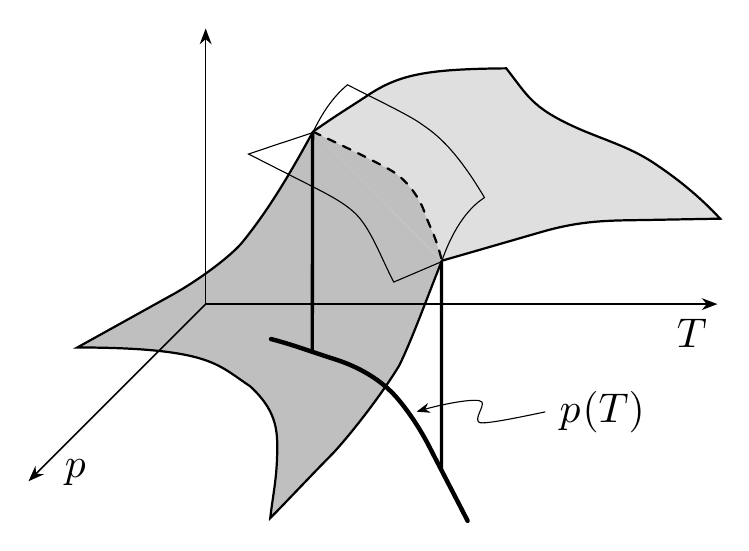
\begin{tikzpicture}[
    line cap=round,>=Stealth,
    every node/.style={scale=1.5}
]
\def\intersection{(1.363,2.19)
.. controls (1.69,2.033) and (2.005,1.889) .. (2.328,1.713)
.. controls (2.59,1.57) and (2.738,1.294) .. (2.782,1.16)
.. controls (2.845,0.972) and (2.917,0.885) .. (3.000,0.551)}
\def\pathA{(1.363,2.19)
  .. controls (1.165,1.83) and (0.848,1.252) .. (0.465,0.785)
  .. controls (0.322,0.61) and (-0.088,0.305) .. (-0.412,0.125)
  .. controls (-0.818,-0.1) and (-1.224,-0.326) .. (-1.63,-0.551)
  .. controls (-1.225,-0.551) and (-0.763,-0.565) .. (-0.412,-0.618)
  .. controls (0.141,-0.701) and (0.263,-0.842) .. (0.565,-1.044)
  .. controls (0.879,-1.332) and (0.912,-1.571) .. (0.909,-1.837)
  .. controls (0.907,-2.207) and (0.858,-2.393) .. (0.82,-2.718)
  .. controls (1.081,-2.453) and (1.33,-2.185) .. (1.592,-1.92)
  .. controls (1.753,-1.758) and (2.198,-1.211) .. (2.46,-0.777)
  .. controls (2.63,-0.427) and (2.822,0.108) .. (3.000,0.551)}
\def\pathB{(3.000,0.551)
  .. controls (3.426,0.673) and (3.849,0.796) .. (4.272,0.918)
  .. controls (4.79,1.068) and (5.146,1.061) .. (5.591,1.068)
  .. controls (5.905,1.074) and (6.219,1.079) .. (6.534,1.085)
  .. controls (6.274,1.365) and (5.984,1.6) .. (5.674,1.803)
  .. controls (5.367,2.004) and (5.023,2.098) .. (4.697,2.245)
  .. controls (4.129,2.503) and (4.087,2.654) .. (3.817,2.994) 
  .. controls (2.809,2.985) and (2.462,2.918) .. (2.063,2.654)
  .. controls (1.853,2.514) and (1.7,2.426) .. (1.363,2.19)}
\fill[gray!50] \pathA \intersection --cycle;
\fill[gray!25] \pathB \intersection --cycle;
\draw[thick] \pathA \pathB;
\draw[] (1.801,2.785)
.. controls (1.612,2.629) and (1.472,2.414) .. (1.361,2.178)
.. controls (1.089,2.088) and (0.816,1.997) .. (0.544,1.906)
.. controls (0.815,1.768) and (1.086,1.63) .. (1.357,1.493)
.. controls (1.633,1.352) and (1.844,1.237) .. (1.972,1.071)
.. controls (2.135,0.861) and (2.25,0.543) .. (2.389,0.28)
.. controls (2.592,0.366) and (2.794,0.453) .. (2.996,0.539)
.. controls (3.153,0.996) and (3.365,1.243) .. (3.541,1.352)
.. controls (3.133,2.042) and (2.869,2.196) .. (2.719,2.301)
.. controls (2.569,2.407) and (2.108,2.627) .. (1.801,2.785)
-- cycle;
\draw[semithick,->] (0,0) -- (6.5,0) node[pos=0.95,below] {$T$};
\draw[semithick,->] (0,0) -- (0,3.5) node[pos=0.9,left] {$\upmu$};
\draw[semithick,->] (0,0) -- (-2.25,-2.25) node[pos=0.95,right=3pt] {$p$};
\draw[dashed,thick] \intersection;
\draw[ultra thick] (0.83,-0.444)
.. controls (1.109,-0.515) and (1.372,-0.616) .. (1.643,-0.701)
.. controls (1.947,-0.798) and (2.228,-0.961) .. (2.423,-1.184)
.. controls (2.56,-1.34) and (2.721,-1.577) .. (2.843,-1.816)
.. controls (2.964,-2.053) and (3.167,-2.441) .. (3.327,-2.753);
\draw[very thick] (1.358,2.175) -- (1.354,-0.6) (2.995,0.536) -- (2.995,-2.096);
\draw[thin,<-] (2.679,-1.366)
.. controls (3.005,-1.271) and (3.465,-1.18) .. (3.508,-1.243)
.. controls (3.544,-1.296) and (3.403,-1.46) .. (3.474,-1.502)
.. controls (3.535,-1.537) and (4.11,-1.41) .. (4.308,-1.37) node[right] {$p_{\upalpha\upbeta}(T)$};
\path
(1.255,-1.513) node {$\upalpha$}
(5.055,1.509) node {$\upbeta$};
\end{tikzpicture}
\end{document}